\documentclass[letterpaper,10pt,onecolumn,titlepage]{article}
 
% Se cargan los paquetes necesarios
\usepackage{verbatim}
\usepackage{mathrsfs}
\usepackage{amsmath}
\usepackage{amssymb}
\usepackage{subfigure}
\usepackage{ucs}
\usepackage[utf8x]{inputenc}
\usepackage[spanish]{babel}
\usepackage{fontenc}
\usepackage{graphicx}
\usepackage{anysize}
\usepackage{xcolor}
\marginsize{2cm}{2cm}{1cm}{1cm}
\usepackage{fancyhdr}
\pagestyle{fancy}
\setlength{\headheight}{13.1pt}
 
% Portada
\author{Andrés Pelaez 2010735004-4 \\ Aníbal Silva 201073524-9}
\title{\begin{Huge}
Redes de Computadores\\
    No somos nada, hola Internet\\
\end{Huge}
    ~\\
    ~\\
    ~\\
    \emph{Tarea Nº3}}
    
\date{20 de Junio de 2014}
 
\begin{document}
 
% Se aplica el formato a las páginas. Se despliegan: portada e índices de materias, figuras y tablas
\renewcommand{\listtablename}{Índice de tablas}
\renewcommand{\tablename}{Tabla}
\maketitle
\setcounter{page}{2}
\tableofcontents{}
%\thispagestyle{empty}
%\newpage
%\listoffigures{}
%\listoftables
\thispagestyle{empty}
\newpage
\fancyhead{}
\fancyfoot{}
 
% Encabezado y pie de página
\lhead{ILI-256 Redes de Computadores}
\lfoot{Tarea 3, No somos nada, hola Internet}
\rfoot{\thepage}
 
% Desarrollo de los contenidos del documento
\section{Tarea 1}
 
Como se solicita en el enunciado, a través del programa \textit{Open Visual TraceRoute} se han calculado las rutas que siguen los paquetes en base a las direcciones señaladas. En la sección Apéndice se encuentran los “pantallazos” de cada una de estas, en donde se muestra con más detalle lo sucedido. \\

A continuación se presenta una tabla con algunos resultados para cada una de las direcciones:

\begin{center}

   \begin{tabular}{|c|c|c|c|} \hline
     Dirección & Num. Países & Num IPs & Largo Ruta [km] \\ \hline
     Moodle    & 1           & 9       & 676             \\ \hline
     Google    & 2           & 3       & 9.196           \\ \hline
     CIME      & 2           & 12      & 17.451          \\ \hline
     Wikipedia & 4           & 6       & 26.334          \\ \hline
     Embajada *  & 4           & 6       & 26.392               \\ \hline
   \end{tabular}\\
   
   \textit{\textbf{Tabla 1:} muestra las 5 direcciones a analizar con la cantidad de países que visita, la cantidad de enrutadores por los que debe pasar (IPs) y el largo total de trayecto.}
 \end{center}

De la anterior tabla rápidamente se obtienen algunas conclusiones:

\begin{itemize}

 \item La cantidad de países por los que debe pasar el paquete no tiene relación con la cantidad de enrutadores. El paquete que va hacia la primera dirección sólo se mueve dentro de Chile, mas debe pasar por 9 diferentes routers, mientras que el paquete que va a la cuarta dirección pasa sólo por 6, pero visita más países (4).

 \item El largo final de la ruta corresponde a la distancia total que tuvo que recorrer el paquete para llegar a su destino, por lo cual si el emisor y receptor están cerca físicamente, el largo de la ruta debería ser bajo. Esto se ejemplifica en la dirección uno, en donde recorre menos de mil kilómetros. Caso contrario para las demás, en donde debe moverse largas distancias. Este hecho era bastante predecible ya que las distancias entre países son muy grandes.
 
 \item Algunas distancias recorridas entre enrutadores muchas veces tienden a cero (para mayor detalle ver figuras en sección Apéndice), pero estas siempre están en el mismo país, por lo cual se deduce que son pequeños enlaces (distancias) que deben hacerse. A pesar de ser distancias cortas, generan tiempos de latencia iguales (o mayores) que distancias largas, lo mismo para la cantidad de DNS lookup que deben realizar.
 
 \item * Es necesario señalar que el programa no ha podido completar la ruta del paquete que se dirigía a la dirección web de la embajada de Chile en Australia. En diferentes ocaciones, el último nodo que alcanzaba también era diferente, siendo en este caso uno ubicado en Japón.
 
\end{itemize}

\noindent \textbf{¿Por qué toman estas rutas los paquetes?} \\

Como se sabe, la información se envía desde un host a otro a través de una gran red de dispositivos conectados entre si, por lo cual los paquetes pasan por estos para llegar a su destino. Ahora bien, el hecho de por qué los paquetes toman los caminos que toman es el siguiente: cada vez que uno llega a un enrutador, este debe observar la dirección IP de destino que se encuentra en la capa de red, y luego compara esta con su tabla de enrutamiento para decidir por cual puerto debe ser enviado. Es así cómo se va generando esta ruta desde un nodo al siguiente hasta llegar al host. \\

\noindent \textbf{¿Cómo viajan de un lugar a otro (continentes)?} \\

Respecto a la red de enrutadores mencionada anteriormente, esta es cableada (o satelital) desde un nodo a otro. Esto es lo que permite que físicamente pueda enviarse información a través de un punto físico completamente distante de otro, ya que es relativamente sencillo transportar señales por un medio cableado, inclusive entre continentes. Claramente esta vía no aplica al momento que un host se conecta de forma inalámbrica a una acces point. \\

\noindent \textbf{Enlaces Internacionales} \\

Actualmente se encuentran en servicio 4 enlaces a internet, más 2 que se planean implementar. En servicio son los siguientes:

\begin{itemize}
 \item South America-1 (SAm-1), Arica.
 \item South America-1 (SAm-1), Valparaíso.
 \item South America Crossing (SAC) / Latin America Nautilus (LAN), Valparaíso.
 \item Pan American (PAN-AM), Arica.
\end{itemize}

Mientras los que se planean implementar son:

\begin{itemize}
 \item Quellon-Puerto Chacabuco, Quellón.
 \item Quellon-Puerto Chacabuco, Puerto Chacabuco.
\end{itemize}

%%\newpage

\section{Tarea 2}

Como se presenta en el enunciado de la tarea 2, un sistema compuesto por 9 routers conectan un PC con un servidor. Utilizando el algoritmo de \textit{vector-distancia}, asignando una tabla especial a cada vector, se procede a efectuar el desarrollo del mismo, donde se deben realizar 11x11 operaciones en cada paso (Hop) que se efectué hasta donde converge la función. Se habla de 11 x 11 porque se incluyeron los vectores de PC y Servidor, pese a que estos valores serán iguales a los del vector A más la distancia del PC al mismo, y los del vector I más la distancia del servidor al nodo I respectivamente. Esto, porque la única conexión que tienen es con los vectores antes mencionados.


\begin{center}
   \begin{tabular}{|c|c|c|c|c|c|c|c|c|c|c|c|} \hline
     MA & A  & B & C & D & E & F & G & H & I  & P & S \\ \hline
     A  & 0  & 1 & - & - & - & - & 4 & - & 10 & 3 & - \\ \hline
     B  & 1  & 0 & 9 & - & 8 & - & - & - & -  & - & - \\ \hline
     C  & -  & 9 & 0 & 2 & - & - & - & - & -  & - & - \\ \hline
     D  & -  & - & 2 & 0 & 9 & 4 & - & - & 2  & - & - \\ \hline
     E  & -  & 8 & - & 9 & 0 & 2 & - & - & 1  & - & - \\ \hline
     F  & -  & - & - & 4 & 2 & 0 & - & 6 & -  & - & - \\ \hline
     G  & 4  & - & - & - & - & - & 0 & 7 & -  & - & - \\ \hline
     H  & -  & - & - & - & - & 6 & 7 & 0 & 3  & - & - \\ \hline
     I  & 10 & - & - & 2 & 1 & - & - & 3 & 0  & - & 1 \\ \hline
     P  & 3  & - & - & - & - & - & - & - & -  & 0 & - \\ \hline
     S  & -  & - & - & - & - & - & - & - & 1  & - & 0 \\ \hline
   \end{tabular}\\
   \textit{\textbf{Tabla 2:} matriz de adyacencia correspondiente a las conexiones existentes entre todos los dispositivos.}
 \end{center}

A continuación se presentarán los pasos realizados del algoritmo Vector-Distancia, en donde cada nodo posee 3 columnas, destina (Ds), costo (Cs) y \textit{Hop Path} (Hp).

\textbf{Hop 1:}

\begin{center}
   \begin{tabular}{|c|c|c|c|c|c|c|c|c|c|c|c|c|c|c|c|c|c|} \hline
    \multicolumn{3}{|c|}{A} & \multicolumn{3}{|c|}{B} & \multicolumn{3}{|c|}{C} & \multicolumn{3}{|c|}{D} & \multicolumn{3}{|c|}{E} & \multicolumn{3}{|c|}{F} \\ \hline
     Ds & Cs & Hp & Ds & Cs & Hp & Ds & Cs & Hp & Ds & Cs & Hp & Ds & Cs & Hp & Ds & Cs & Hp \\ \hline
     A  & 0  & A  & A  & 1  & A  & A  & -  & -  & A  & -  & -  & A  & -  & -  & A  & -  & - \\ \hline
     B  & 1  & B  & B  & 0  & B  & B  & 9  & B  & B  & -  & -  & B  & -  & - & B  & -  & - \\ \hline
     C  & -  & -  & C  & 9  & C  & C  & 0  & C  & C  & 2  & C  & C  & -  & -  & C  & -  & - \\ \hline
     D  & -  & -  & D  & -  & - & D  & 2  & D  & D  & 0  & D  & D  & 9  & D  & D  & 4  & D \\ \hline
     E  & -  & -  & E  & 8  & E  & E  & -  & -  & E  & 9  & E  & E  & 0  & E  & E  & 2  & E \\ \hline
     F  & -  & -  & F  & -  & -  & F  & -  & -  & F  & 4  & F  & F  & 2  & F  & F  & 0  & F \\ \hline
     G  & 4  & G  & G  & -  & -  & G  & -  & -  & G  & -  & -  & G  & -  & -  & G  & -  & - \\ \hline
     H  & -  & -  & H  & -  & -  & H  & -  & -  & H  & -  & -  & H  & -  & -  & H  & 6  & H \\ \hline
     I  & 10  & I  & I  & -  & -  & I  & -  & -  & I  & 2  & I  & I  & 1  & I  & I  & -  & - \\ \hline
     P  & 3  & P  & P  & -  & -  & P  & -  & -  & P  & -  & -  & P  & -  & -  & P  & -  & - \\ \hline
     S  & -  & -  & S  & -  & -  & S  & -  & -  & S  & -  & -  & S  & -  & -  & S  & -  & - \\ \hline
   \end{tabular}\\
   \textit{\textbf{Tabla 3:} primer paso del algoritmo Vector-Distancia aplicado a la red del enunciado.}
 \end{center}
 
  \begin{center}
   \begin{tabular}{|c|c|c|c|c|c|c|c|c|c|c|c|c|c|c|} \hline
     \multicolumn{3}{|c|}{G} & \multicolumn{3}{|c|}{H} &\multicolumn{3}{|c|}{I} & \multicolumn{3}{|c|}{P} & \multicolumn{3}{|c|}{S}    \\ \hline
     Ds & Cs & Hp & Ds & Cs & Hp & Ds & Cs & Hp & Ds & Cs & Hp & Ds & Cs & Hp  \\ \hline
     A  & 4  & A  & A  & -  & -  & A  & 10  & A  & A  & 3  & A  & A  & -  & -   \\ \hline
     B  & -  & -  & B  & -  & -  & B  & -  & -  & B  & -  & -  & B  & -  & -   \\ \hline
     C  & -  & -  & C  & -  & -  & C  & -  & -  & C  & -  & -  & C  & -  & -   \\ \hline
     D  & -  & -  & D  & -  & -  & D  & 2  & D  & D  & -  & -  & D  & -  & -   \\ \hline
     E  & -  & -  & E  & -  & -  & E  & 1  & E  & E  & -  & -  & E  & -  & -   \\ \hline
     F  & -  & -  & F  & 6  & F  & F  & -  & -  & F  & -  & -  & F  & -  & -   \\ \hline
     G  & 0  & G  & G  & 7  & G  & G  & -  & -  & G  & -  & -  & G  & -  & -   \\ \hline
     H  & 7  & H  & H  & 0  & H  & H  & 3  & H  & H  & -  & -  & H  & -  & -   \\ \hline
     I  & -  & -  & I  & 3  & I  & I  & 0  & I  & I  & -  & -  & I  & 1  & I   \\ \hline
     P  & -  & -  & P  & -  & -  & P  & -  & -  & P  & 0  & P  & P  & -  & -   \\ \hline
     S  & -  & -  & S  & -  & -  & S  & 1  & S  & S  & -  & -  & S  & 0  & S   \\ \hline
   \end{tabular}\\
   \textit{\textbf{Tabla 4:} continuación del primer paso del algoritmo Vector-Distancia aplicado a la red del enunciado.}
 \end{center}
 
 \textbf{Hop 2:}
 \begin{center}
   \begin{tabular}{|c|c|c|c|c|c|c|c|c|c|c|c|c|c|c|c|c|c|} \hline
     \multicolumn{3}{|c|}{A} & \multicolumn{3}{|c|}{B} & \multicolumn{3}{|c|}{C} & \multicolumn{3}{|c|}{D} & \multicolumn{3}{|c|}{E} & \multicolumn{3}{|c|}{F} \\ \hline
     Ds & Cs & Hp & Ds & Cs & Hp & Ds & Cs & Hp & Ds & Cs & Hp & Ds & Cs & Hp & Ds & Cs & Hp \\ \hline
     A  & 0  & A  & A  & 1  & A  & A  & 10  & B  & A  & \color{red}12  &\color{red} I  & A  & \color{red}9  & \color{red}B  & A  & -  & - \\ \hline
     B  & 1  & B  & B  & 0  & B  & B  & 9  & B  & B  & \color{red}11  & \color{red}C  & B  & 8  & B & B  & \color{red}10  & \color{red}E \\ \hline
     C  & \color{red}10  &\color{red} B  & C  & 9  & C  & C  & 0  & C  & C  & 2  & C  & C  & \color{red}11  & \color{red}D  & C  & \color{red}6  & \color{red}D \\ \hline
     D  & \color{red}12  & \color{red}I  & D  & \color{red}11  & \color{red}C & D  & \color{red}2  & \color{red}D  & D  & 0  & D  & D  & \color{red}3  & \color{red}I  & D  & 4  & D \\ \hline
     E  & \color{red}9  & \color{red}B  & E  & 8  & E  & E  & \color{red}11  & \color{red}D  & E  & \color{red}3  &\color{red} I  & E  & 0  & E  & E  & 2  & E \\ \hline
     F  & -  & -  & F  & \color{red}10  & \color{red}E  & F  & \color{red}6  & \color{red}D  & F  & 4  & F  & F  & 2  & F  & F  & 0  & F \\ \hline
     G  & 4  & G  & G  & \color{red}5  & \color{red}A  & G  & -  & -  & G  & -  & -  & G  & -  & -  & G  & \color{red}13  & \color{red}H \\ \hline
     H  & \color{red}11  & \color{red}G  & H  & -  & -  & H  & -  & -  & H  & \color{red}5  & \color{red}I  & H  & \color{red}4  &\color{red} I  & H  & 6  & H \\ \hline
     I  & 10  & I  & I  &\color{red} 9  & \color{red}E  & I  & \color{red}4  & \color{red}D  & I  & 2  & I  & I  & 1  & I  & I  & \color{red}3  & \color{red}E \\ \hline
     P  & 3  & P  & P  & \color{red}4  & \color{red}A  & P  & -  & -  & P  & -  & -  & P  & -  & -  & P  & -  & - \\ \hline
     S  & \color{red}11  & \color{red}I  & S  & -  & -  & S  & -  & -  & S  & \color{red}3  &\color{red} I  & S  &\color{red} 2  &\color{red} I  & S  & -  & - \\ \hline
   \end{tabular}\\
   \textit{\textbf{Tabla 5:} segundo paso del algoritmo Vector-Distancia aplicado a la red del enunciado.}
 \end{center}
 
  \begin{center}
   \begin{tabular}{|c|c|c|c|c|c|c|c|c|c|c|c|c|c|c|} \hline
     \multicolumn{3}{|c|}{G} & \multicolumn{3}{|c|}{H} &\multicolumn{3}{|c|}{I} & \multicolumn{3}{|c|}{P} & \multicolumn{3}{|c|}{S}    \\ \hline
     Ds & Cs & Hp & Ds & Cs & Hp & Ds & Cs & Hp & Ds & Cs & Hp & Ds & Cs & Hp  \\ \hline
     A  & 4  & A  & A  & \color{red}11  & \color{red}G  & A  & 10  & A  & A  & 3  & A  & A  & \color{red}11  & \color{red}I   \\ \hline
     B  & \color{red}5  & \color{red}A  & B  & -  & -  & B  & \color{red}9  &\color{red} E  & B  & \color{red}4  & \color{red}A  & B  & -  & -   \\ \hline
     C  & -  & -  & C  & -  & -  & C  & \color{red}4  &\color{red} D  & C  & -  & -  & C  & -  & -   \\ \hline
     D  & -  & -  & D  & \color{red}5  & \color{red}I  & D  & 2  & D  & D  & -  & -  & D  & \color{red}3  &\color{red} I   \\ \hline
     E  & -  & -  & E  & \color{red}4  &\color{red} I  & E  & 1  & E  & E  & -  & -  & E  & \color{red}2  & \color{red}I   \\ \hline
     F  & \color{red}13  & \color{red}H  & F  & 6  & F  & F  & \color{red}3  & \color{red}E  & F  & -  & -  & F  & -  & -   \\ \hline
     G  & 0  & G  & G  & 7  & G  & G  & \color{red}10  & \color{red}H  & G  & \color{red}7  & \color{red}A  & G  & -  & -   \\ \hline
     H  & 7  & H  & H  & 0  & H  & H  & 3  & H  & H  & -  & -  & H  & \color{red}4  &\color{red} I   \\ \hline
     I  & \color{red}10  & \color{red}H  & I  & 3  & I  & I  & 0  & I  & I  & \color{red}13  & \color{red}A  & I  & 1  & I   \\ \hline
     P  & \color{red}7  & \color{red}A  & P  & -  & -  & P  & \color{red}13  & \color{red}A  & P  & 0  & P  & P  & -  & -   \\ \hline
     S  & -  & -  & S  & \color{red}4  &\color{red} I  & S  & 1  & S  & S  & -  & -  & S  & 0  & S   \\ \hline
   \end{tabular}\\
   \textit{\textbf{Tabla 6:} continuación del segundo paso del algoritmo Vector-Distancia aplicado a la red del enunciado.}
 \end{center}
 
\newpage 
 
 \textbf{Hop 3:}
 
 \begin{center}
   \begin{tabular}{|c|c|c|c|c|c|c|c|c|c|c|c|c|c|c|c|c|c|} \hline
    \multicolumn{3}{|c|}{A} & \multicolumn{3}{|c|}{B} & \multicolumn{3}{|c|}{C} & \multicolumn{3}{|c|}{D} & \multicolumn{3}{|c|}{E} & \multicolumn{3}{|c|}{F} \\ \hline
     Ds & Cs & Hp & Ds & Cs & Hp & Ds & Cs & Hp & Ds & Cs & Hp & Ds & Cs & Hp & Ds & Cs & Hp \\ \hline
     A  & 0  & A  & A  & 1  & A  & A  & 10  & B  & A  & 12  & I  & A  & 9  & B  & A  & \color{red}11  & \color{red}E \\ \hline
     B  & 1  & B  & B  & 0  & B  & B  & 9  & B  & B  & 11  & C  & B  & 8  & B & B  & 10  & E \\ \hline
     C  & 10  & B  & C  & 9  & C  & C  & 0  & C  & C  & 2  & C  & C  & \color{red}5  & \color{red}I  & C  & 6  & D \\ \hline
     D  & 12  & I  & D  & 11  & C & D  & 2  & D  & D  & 0  & D  & D  & 3  & I  & D  & 4  & D \\ \hline
     E  & 9  & B  & E  & 8  & E  & E  & \color{red}5  & \color{red}D  & E  & 3  & I  & E  & 0  & E  & E  & 2  & E \\ \hline
     F  & \color{red}11  &\color{red} B  & F  & 10  & E  & F  & 6  & D  & F  & 4  & F  & F  & 2  & F  & F  & 0  & F \\ \hline
     G  & 4  & G  & G  & 5  & A  & G  & \color{red}14  & \color{red}B  & G  & \color{red}12  & \color{red}I  & G  & \color{red}11  &\color{red} I  & G  & 13  & H \\ \hline
     H  & 11  & G  & H  & \color{red}12  & \color{red}A  & H  & \color{red}7  & \color{red}D  & H  & 5  & I  & H  & 4  & I  & H  & 6  & H \\ \hline
     I  & 10  & I  & I  & 9  & E  & I  & 4  & D  & I  & 2  & I  & I  & 1  & I  & I  & 3  & E \\ \hline
     P  & 3  & P  & P  & 4  & A  & P  & \color{red}13  & \color{red}B  & P  & \color{red}15  & \color{red}I  & P  & \color{red}12  & \color{red}B  & P  & -  & - \\ \hline
     S  & 11  & I  & S  & \color{red}10  &\color{red} E  & S  & \color{red}5  & \color{red}D  & S  & 3  & I  & S  & 2  & I  & S  & \color{red}4  & \color{red}E \\ \hline
   \end{tabular}\\
   \textit{\textbf{Tabla 7:} tercer paso del algoritmo Vector-Distancia aplicado a la red del enunciado.}
 \end{center}
 
  \begin{center}
   \begin{tabular}{|c|c|c|c|c|c|c|c|c|c|c|c|c|c|c|} \hline
     \multicolumn{3}{|c|}{G} & \multicolumn{3}{|c|}{H} &\multicolumn{3}{|c|}{I} & \multicolumn{3}{|c|}{P} & \multicolumn{3}{|c|}{S}    \\ \hline
     Ds & Cs & Hp & Ds & Cs & Hp & Ds & Cs & Hp & Ds & Cs & Hp & Ds & Cs & Hp  \\ \hline
     A  & 4  & A  & A  & 11  & G  & A  & 10  & A  & A  & 3  & A  & A  & 11  & I   \\ \hline
     B  & 5  & A  & B  & \color{red}12  & \color{red}G  & B  & 9  & E  & B  & 4  & A  & B  & \color{red}10  &\color{red} I   \\ \hline
     C  & \color{red}14  & \color{red}A  & C  & \color{red}7  & \color{red}I  & C  & 4  & D  & C  &\color{red} 13  &\color{red} A  & C  & \color{red}5  & \color{red}I   \\ \hline
     D  & \color{red}12  & \color{red}H  & D  & 5  & I  & D  & 2  & D  & D  & \color{red}15  & \color{red}A  & D  & 3  & I   \\ \hline
     E  & \color{red}11  & \color{red}H  & E  & 4  & I  & E  & 1  & E  & E  & \color{red}12  &\color{red} A  & E  & 2  & I   \\ \hline
     F  & 13  & H  & F  & 6  & F  & F  & 3  & E  & F  & -  & -  & F  & \color{red}4  & \color{red}I   \\ \hline
     G  & 0  & G  & G  & 7  & G  & G  & 10  & H  & G  & 7  & A  & G  & \color{red}11  &\color{red} I   \\ \hline
     H  & 7  & H  & H  & 0  & H  & H  & 3  & H  & H  & \color{red}14  & \color{red}A  & H  & 4  & I   \\ \hline
     I  & 10  & H  & I  & 3  & I  & I  & 0  & I  & I  & 13  & A  & I  & 1  & I   \\ \hline
     P  & 7  & A  & P  & \color{red}14  & \color{red}G  & P  & 13  & A  & P  & 0  & P  & P  & \color{red}14  &\color{red} I \\ \hline
     S  & \color{red}11  &\color{red} H  & S  & 4  & I  & S  & 1  & S  & S  & \color{red}14  & \color{red}A  & S  & 0  & S   \\ \hline
   \end{tabular}\\
   \textit{\textbf{Tabla 8:} continuación del tercer paso del algoritmo Vector-Distancia aplicado a la red del enunciado.}
 \end{center}
 
 \textbf{Hop 4:}
 
 \begin{center}
   \begin{tabular}{|c|c|c|c|c|c|c|c|c|c|c|c|c|c|c|c|c|c|} \hline
     \multicolumn{3}{|c|}{A} & \multicolumn{3}{|c|}{B} & \multicolumn{3}{|c|}{C} & \multicolumn{3}{|c|}{D} & \multicolumn{3}{|c|}{E} & \multicolumn{3}{|c|}{F} \\ \hline
     Ds & Cs & Hp & Ds & Cs & Hp & Ds & Cs & Hp & Ds & Cs & Hp & Ds & Cs & Hp & Ds & Cs & Hp \\ \hline
     A  & 0  & A  & A  & 1  & A  & A  & 10  & B  & A  & 12  & I  & A  & 9  & B  & A  & 11  & E \\ \hline
     B  & 1  & B  & B  & 0  & B  & B  & 9  & B  & B  & 11  & C  & B  & 8  & B & B  & 10  & E \\ \hline
     C  & 10  & B  & C  & 9  & C  & C  & 0  & C  & C  & 2  & C  & C  & 5  & I  & C  & 6  & D \\ \hline
     D  & 12  & I  & D  & 11  & C & D  & 2  & D  & D  & 0  & D  & D  & 3  & I  & D  & 4  & D \\ \hline
     E  & 9  & B  & E  & 8  & E  & E  & 5  & D  & E  & 3  & I  & E  & 0  & E  & E  & 2  & E \\ \hline
     F  & 11  & B  & F  & 10  & E  & F  & 6  & D  & F  & 4  & F  & F  & 2  & F  & F  & 0  & F \\ \hline
     G  & 4  & G  & G  & 5  & A  & G  & 14  & b  & G  & 12  & I  & G  & 11  & I  & G  & 13  & H \\ \hline
     H  & 11  & G  & H  & 12  & A  & H  & 7  & D  & H  & 5  & I  & H  & 4  & I  & H  & 6  & H \\ \hline
     I  & 10  & I  & I  & 9  & E  & I  & 4  & D  & I  & 2  & I  & I  & 1  & I  & I  & 3  & E \\ \hline
     P  & 3  & P  & P  & 4  & A  & P  & 13  & B  & P  & 15  & I  & P  & 12  & B  & P  & \color{red}14  & \color{red}E \\ \hline
     S  & 11  & I  & S  & 10  & E  & S  & 5  & D  & S  & 3  & I  & S  & 2  & I  & S  & 4  & E \\ \hline
   \end{tabular}\\
   \textit{\textbf{Tabla 9:} cuarto paso del algoritmo Vector-Distancia aplicado a la red del enunciado.}
 \end{center}
 
  \begin{center}
   \begin{tabular}{|c|c|c|c|c|c|c|c|c|c|c|c|c|c|c|} \hline
     \multicolumn{3}{|c|}{G} & \multicolumn{3}{|c|}{H} &\multicolumn{3}{|c|}{I} & \multicolumn{3}{|c|}{P} & \multicolumn{3}{|c|}{S}    \\ \hline
     Ds & Cs & Hp & Ds & Cs & Hp & Ds & Cs & Hp & Ds & Cs & Hp & Ds & Cs & Hp  \\ \hline
     A  & 4  & A  & A  & 11  & G  & A  & 10  & A  & A  & 3  & A  & A  & 11  & I   \\ \hline
     B  & 5  & A  & B  & 12  & G  & B  & 9  & E  & B  & 4  & A  & B  & 10  & I   \\ \hline
     C  & 14  & A  & C  & 7  & I  & C  & 4  & D  & C  & 13  & A  & C  & 5  & I   \\ \hline
     D  & 12  & H  & D  & 5  & I  & D  & 2  & D  & D  & 15  & A  & D  & 3  & I   \\ \hline
     E  & 11  & H  & E  & 4  & I  & E  & 1  & E  & E  & 12  & A  & E  & 2  & I   \\ \hline
     F  & 13  & H  & F  & 6  & F  & F  & 3  & E  & F  & \color{red}14  &\color{red} A  & F  & 4  & I   \\ \hline
     G  & 0  & G  & G  & 7  & G  & G  & 10  & H  & G  & 7  & A  & G  & 11  & I   \\ \hline
     H  & 7  & H  & H  & 0  & H  & H  & 3  & H  & H  & 14  & A  & H  & 4  & I   \\ \hline
     I  & 10  & H  & I  & 3  & I  & I  & 0  & I  & I  & 13  & A  & I  & 1  & I   \\ \hline
     P  & 7  & A  & P  & 14  & G  & P  & 13  & A  & P  & 0  & P  & P  & 14  & I \\ \hline
     S  & 11  & H  & S  & 4  & I  & S  & 1  & S  & S  & 14  & A  & S  & 0  & S   \\ \hline
   \end{tabular}\\
   \textit{\textbf{Tabla 10:} continuación del cuarto paso del algoritmo Vector-Distancia aplicado a la red del enunciado.}
 \end{center}
 
Como se anticipó en un comienzo, las tablas P y S vienen a ser la tabla A sumado a 3 (costo del PC a vector A) e I sumado a 1 (costo del Servidor al vector I), además lo que garantiza este algoritmo vector-distancia es que estas son las distancias mínimas de cada vector o router hasta el destino especificado, además de mostrar los caminos por los cuales transita la señal (Hop o Hp). Así, se puede observar que observando la tabla del vector P o PC, la distancia mínima al servidor es de costo 14, siguiendo el siguiente camino: A (3) $\to$ I (10) $\to$ S (1).
%%\newpage

\section{Tarea 3}

Lo efectuado en esta sección, es igual a lo hecho en la pregunta 2, con el cambio que se ha eliminado la conexión entre H-I, así las rutas que usaban dicho enlace deben buscar otra ruta para poder llegar al servidor, no existe tipo de optimización alguna, ya que siendo un enlace relativamente de bajo costo (para el total del mapa entero), solo provoca aumentos de costo en la mayoría de los vectores, no así el caso de D-E donde es un enlace que termina por no utilizarse en ninguna de las dos ocasiones, ya que tiene una alternativa de bajo costo por el vector I.

\begin{center}
   \begin{tabular}{|c|c|c|c|c|c|c|c|c|c|c|c|} \hline
     MA & A  & B & C & D & E & F & G & H & I  & P & S \\ \hline
     A  & 0  & 1 & - & - & - & - & 4 & - & 10 & 3 & - \\ \hline
     B  & 1  & 0 & 9 & - & 8 & - & - & - & -  & - & - \\ \hline
     C  & -  & 9 & 0 & 2 & - & - & - & - & -  & - & - \\ \hline
     D  & -  & - & 2 & 0 & 9 & 4 & - & - & 2  & - & - \\ \hline
     E  & -  & 8 & - & 9 & 0 & 2 & - & - & 1  & - & - \\ \hline
     F  & -  & - & - & 4 & 2 & 0 & - & 6 & -  & - & - \\ \hline
     G  & 4  & - & - & - & - & - & 0 & 7 & -  & - & - \\ \hline
     H  & -  & - & - & - & - & 6 & 7 & 0 & -  & - & - \\ \hline
     I  & 10 & - & - & 2 & 1 & - & - & - & 0  & - & 1 \\ \hline
     P  & 3  & - & - & - & - & - & - & - & -  & 0 & - \\ \hline
     S  & -  & - & - & - & - & - & - & - & 1  & - & 0 \\ \hline
   \end{tabular}\\
   \textit{\textbf{Tabla 11:} matriz de adyacencia correspondiente a las conexiones existentes entre todos los dispositivos, menos conexión entre nodos H e I.}
 \end{center}

\newpage

\textbf{Hop 1:}
 \begin{center}
   \begin{tabular}{|c|c|c|c|c|c|c|c|c|c|c|c|c|c|c|c|c|c|} \hline
    \multicolumn{3}{|c|}{A} & \multicolumn{3}{|c|}{B} & \multicolumn{3}{|c|}{C} & \multicolumn{3}{|c|}{D} & \multicolumn{3}{|c|}{E} & \multicolumn{3}{|c|}{F} \\ \hline
     Ds & Cs & Hp & Ds & Cs & Hp & Ds & Cs & Hp & Ds & Cs & Hp & Ds & Cs & Hp & Ds & Cs & Hp \\ \hline
     A  & 0  & A  & A  & 1  & A  & A  & 10  & B  & A  & -  & -  & A  & -  & -  & A  & -  & - \\ \hline
     B  & 1  & B  & B  & 0  & B  & B  & 9  & B  & B  & -  & -  & B  & 8  & B & B  & -  & - \\ \hline
     C  & 10  & B  & C  & 9  & C  & C  & 0  & C  & C  & 2  & C  & C  & -  & -  & C  & -  & - \\ \hline
     D  & 12  & I  & D  & 11  & C & D  & 2  & D  & D  & 0  & D  & D  & 9  & D  & D  & -  & - \\ \hline
     E  & 9  & B  & E  & 8  & E  & E  & 11  & D  & E  & 9  & E  & E  & 0  & E  & E  & 2  & E \\ \hline
     F  & -  & -  & F  & 10  & E  & F  & 6  & D  & F  & 4  & F  & F  & 2  & F  & F  & 0  & F \\ \hline
     G  & 4  & G  & G  & 5  & A  & G  & -  & -  & G  & -  & -  & G  & -  & -  & G  & -  & - \\ \hline
     H  & 11  & G  & H  & -  & -  & H  & -  & -  & H  & -  & -  & H  & -  & -  & H  & 6  & H \\ \hline
     I  & 10  & I  & I  & 9  & E  & I  & 4  & D  & I  & 2  & I  & I  & 1  & I  & I  & -  & - \\ \hline
     P  & 3  & P  & P  & 4  & A  & P  & -  & -  & P  & -  & -  & P  & -  & -  & P  & -  & - \\ \hline
     S  & 11  & I  & S  & -  & -  & S  & -  & -  & S  & -  & -  & S  & -  & -  & S  & -  & - \\ \hline
   \end{tabular}\\
   \textit{\textbf{Tabla 12:} primer paso del algoritmo Vector-Distancia aplicado a la red del enunciado, no considerando arco H-I.}
 \end{center}
 
  \begin{center}
   \begin{tabular}{|c|c|c|c|c|c|c|c|c|c|c|c|c|c|c|} \hline
     \multicolumn{3}{|c|}{G} & \multicolumn{3}{|c|}{H} &\multicolumn{3}{|c|}{I} & \multicolumn{3}{|c|}{P} & \multicolumn{3}{|c|}{S}    \\ \hline
     Ds & Cs & Hp & Ds & Cs & Hp & Ds & Cs & Hp & Ds & Cs & Hp & Ds & Cs & Hp  \\ \hline
     A  & 4  & A  & A  & -  & -  & A  & 10  & A  & A  & 3  & A  & A  & -  & -   \\ \hline
     B  & -  & -  & B  & -  & -  & B  & -  & -  & B  & -  & -  & B  & -  & -   \\ \hline
     C  & -  & -  & C  & -  & -  & C  & -  & -  & C  & -  & -  & C  & -  & -   \\ \hline
     D  & -  & -  & D  & -  & -  & D  & 2  & D  & D  & -  & -  & D  & -  & -   \\ \hline
     E  & -  & -  & E  & -  & -  & E  & 1  & E  & E  & -  & -  & E  & -  & -   \\ \hline
     F  & -  & -  & F  & 6  & F  & F  & -  & -  & F  & -  & -  & F  & -  & -   \\ \hline
     G  & 0  & G  & G  & 7  & G  & G  & -  & -  & G  & -  & -  & G  & -  & -   \\ \hline
     H  & 7  & H  & H  & 0  & H  & H  & -  & -  & H  & -  & -  & H  & -  & -   \\ \hline
     I  & -  & -  & I  & -  & -  & I  & 0  & I  & I  & -  & -  & I  & 1  & I   \\ \hline
     P  & -  & -  & P  & -  & -  & P  & -  & -  & P  & 0  & P  & P  & -  & -   \\ \hline
     S  & -  & -  & S  & -  & -  & S  & 1  & S  & S  & -  & -  & S  & 0  & S   \\ \hline
   \end{tabular}\\
   \textit{\textbf{Tabla 13:} continuación del primer paso del algoritmo Vector-Distancia aplicado a la red del enunciado, no considerando arco H-I.}
 \end{center}
 
\textbf{Hop 2:}
 \begin{center}
   \begin{tabular}{|c|c|c|c|c|c|c|c|c|c|c|c|c|c|c|c|c|c|} \hline
     \multicolumn{3}{|c|}{A} & \multicolumn{3}{|c|}{B} & \multicolumn{3}{|c|}{C} & \multicolumn{3}{|c|}{D} & \multicolumn{3}{|c|}{E} & \multicolumn{3}{|c|}{F} \\ \hline
     Ds & Cs & Hp & Ds & Cs & Hp & Ds & Cs & Hp & Ds & Cs & Hp & Ds & Cs & Hp & Ds & Cs & Hp \\ \hline
     A  & 0  & A  & A  & 1  & A  & A  & 10  & B  & A  & \color{red}12  & \color{red}I  & A  & \color{red}9  & \color{red}B  & A  & -  & - \\ \hline
     B  & 1  & B  & B  & 0  & B  & B  & 9  & B  & B  & \color{red}11  &\color{red} C  & B  & 8  & B & B  & \color{red}10  &\color{red} E \\ \hline
     C  & \color{red}10  & \color{red}B  & C  & 9  & C  & C  & 0  & C  & C  & 2  & C  & C  & \color{red}11  & \color{red}D  & C  &\color{red} 6  &\color{red} D \\ \hline
     D  & \color{red}12  &\color{red} I  & D  & \color{red}11  & \color{red}C & D  & \color{red}2  &\color{red} D  & D  & 0  & D  & D  & \color{red}3  & \color{red}I  & D  & 4  & D \\ \hline
     E  &\color{red} 9  & \color{red}B  & E  & 8  & E  & E  & \color{red}11  &\color{red} D  & E  & \color{red}3  &\color{red} I  & E  & 0  & E  & E  & 2  & E \\ \hline
     F  & -  & -  & F  & \color{red}10  & \color{red}E  & F  & \color{red}6  &\color{red} D  & F  & 4  & F  & F  & 2  & F  & F  & 0  & F \\ \hline
     G  & 4  & G  & G  & \color{red}5  & \color{red}A  & G  & -  & -  & G  & -  & -  & G  & -  & -  & G  & \color{red}13  & \color{red}H \\ \hline
     H  & \color{red}11  & \color{red}G  & H  & -  & -  & H  & -  & -  & H  & \color{red}10  &\color{red} F  & H  & \color{red}8  & \color{red}F  & H  & 6  & H \\ \hline
     I  & 10  & I  & I  & \color{red}9  & \color{red}E  & I  & \color{red}4  & \color{red}D  & I  & 2  & I  & I  & 1  & I  & I  & \color{red}3  & \color{red}E \\ \hline
     P  & 3  & P  & P  & \color{red}4  & \color{red}A  & P  & -  & -  & P  & -  & -  & P  & -  & -  & P  & -  & - \\ \hline
     S  &\color{red} 11  &\color{red} I  & S  & -  & -  & S  & -  & -  & S  & \color{red}3  & \color{red}I  & S  &\color{red} 2  & \color{red}I  & S  & -  & - \\ \hline
   \end{tabular}\\
   \textit{\textbf{Tabla 14:} segundo paso del algoritmo Vector-Distancia aplicado a la red del enunciado, no considerando arco H-I.}
 \end{center}
 
  \begin{center}
   \begin{tabular}{|c|c|c|c|c|c|c|c|c|c|c|c|c|c|c|} \hline
     \multicolumn{3}{|c|}{G} & \multicolumn{3}{|c|}{H} &\multicolumn{3}{|c|}{I} & \multicolumn{3}{|c|}{P} & \multicolumn{3}{|c|}{S}    \\ \hline
     Ds & Cs & Hp & Ds & Cs & Hp & Ds & Cs & Hp & Ds & Cs & Hp & Ds & Cs & Hp  \\ \hline
     A  & 4  & A  & A  & \color{red}11  &\color{red} G  & A  & 10  & A  & A  & 3  & A  & A  & \color{red}11  &\color{red} I   \\ \hline
     B  & \color{red}5  & \color{red}A  & B  & -  & -  & B  & \color{red}9  & \color{red}E  & B  &\color{red} 4  & \color{red}A  & B  & -  & -   \\ \hline
     C  & -  & -  & C  & -  & -  & C  & \color{red}4  & \color{red}D  & C  & -  & -  & C  & -  & -   \\ \hline
     D  & -  & -  & D  & \color{red}10  & \color{red}F  & D  & 2  & D  & D  & -  & -  & D  &\color{red} 3  &\color{red} I   \\ \hline
     E  & -  & -  & E  & \color{red}8  & \color{red}F  & E  & 1  & E  & E  & -  & -  & E  & \color{red}2  &\color{red} I   \\ \hline
     F  & \color{red}13  & \color{red}H  & F  & 6  & F  & F  & \color{red}3  &\color{red} E  & F  & -  & -  & F  & -  & -   \\ \hline
     G  & 0  & G  & G  & 7  & G  & G  & \color{red}14  & \color{red}A  & G  & \color{red}7  & \color{red}A  & G  & -  & -   \\ \hline
     H  & 7  & H  & H  & 0  & H  & H  & -  & -  & H  & -  & -  & H  & -  & -   \\ \hline
     I  & \color{red}14  & \color{red}A  & I  & -  & -  & I  & 0  & I  & I  & \color{red}13  & \color{red}A  & I  & 1  & I   \\ \hline
     P  & \color{red}7  & \color{red}A  & P  & -  & -  & P  & \color{red}13  &\color{red} A  & P  & 0  & P  & P  & -  & -   \\ \hline
     S  & -  & -  & S  & -  & -  & S  & 1  & S  & S  & -  & -  & S  & 0  & S   \\ \hline
   \end{tabular}\\
   \textit{\textbf{Tabla 15:} continuación del segundo paso del algoritmo Vector-Distancia aplicado a la red del enunciado, no considerando arco H-I.}
 \end{center}

\textbf{Hop 3:}
 \begin{center}
   \begin{tabular}{|c|c|c|c|c|c|c|c|c|c|c|c|c|c|c|c|c|c|} \hline
     \multicolumn{3}{|c|}{A} & \multicolumn{3}{|c|}{B} & \multicolumn{3}{|c|}{C} & \multicolumn{3}{|c|}{D} & \multicolumn{3}{|c|}{E} & \multicolumn{3}{|c|}{F} \\ \hline
     Ds & Cs & Hp & Ds & Cs & Hp & Ds & Cs & Hp & Ds & Cs & Hp & Ds & Cs & Hp & Ds & Cs & Hp \\ \hline
     A  & 0  & A  & A  & 1  & A  & A  & 10  & B  & A  & 12  & I  & A  & 9  & B  & A  & \color{red}11  & \color{red}E \\ \hline
     B  & 1  & B  & B  & 0  & B  & B  & 9  & B  & B  & 11  & C  & B  & 8  & B & B  & 10  & E \\ \hline
     C  & 10  & B  & C  & 9  & C  & C  & 0  & C  & C  & 2  & C  & C  &\color{red} 5  & \color{red}I  & C  & 6  & D \\ \hline
     D  & 12  & I  & D  & 11  & C & D  & 2  & D  & D  & 0  & D  & D  & 3  & I  & D  & 4  & D \\ \hline
     E  & 9  & B  & E  & 8  & E  & E  &\color{red} 5  & \color{red}D  & E  & 3  & I  & E  & 0  & E  & E  & 2  & E \\ \hline
     F  &\color{red} 11  & \color{red}B  & F  & 10  & E  & F  & 6  & D  & F  & 4  & F  & F  & 2  & F  & F  & 0  & F \\ \hline
     G  & 4  & G  & G  & 5  & A  & G  & \color{red}14  & \color{red}B  & G  &\color{red} 16  &\color{red} I  & G  & \color{red}13  &\color{red} B  & G  & 13  & H \\ \hline
     H  & 11  & G  & H  & \color{red}12  & \color{red}A  & H  & \color{red}12  & \color{red}D  & H  & 10  & F  & H  & 8  & F  & H  & 6  & H \\ \hline
     I  & 10  & I  & I  & 9  & E  & I  & 4  & D  & I  & 2  & I  & I  & 1  & I  & I  & 3  & E \\ \hline
     P  & 3  & P  & P  & 4  & A  & P  & \color{red}13  & \color{red}B  & P  & \color{red}15  &\color{red} I  & P  & \color{red}12  & \color{red}B  & P  & -  & - \\ \hline
     S  & 11  & I  & S  & \color{red}10  & \color{red}E  & S  & \color{red}5  & \color{red}D  & S  & 3  & I  & S  & 2  & I  & S  & \color{red}4  & \color{red}E \\ \hline
   \end{tabular}\\
   \textit{\textbf{Tabla 16:} tercer paso del algoritmo Vector-Distancia aplicado a la red del enunciado, no considerando arco H-I.}
 \end{center}
 
  \begin{center}
   \begin{tabular}{|c|c|c|c|c|c|c|c|c|c|c|c|c|c|c|} \hline
     \multicolumn{3}{|c|}{G} & \multicolumn{3}{|c|}{H} &\multicolumn{3}{|c|}{I} & \multicolumn{3}{|c|}{P} & \multicolumn{3}{|c|}{S}    \\ \hline
     Ds & Cs & Hp & Ds & Cs & Hp & Ds & Cs & Hp & Ds & Cs & Hp & Ds & Cs & Hp  \\ \hline
     A  & 4  & A  & A  & 11  & G  & A  & 10  & A  & A  & 3  & A  & A  & 11  & I   \\ \hline
     B  & 5  & A  & B  & \color{red}12  & \color{red}G  & B  & 9  & E  & B  & 4  & A  & B  & \color{red}10  &\color{red} I   \\ \hline
     C  & \color{red}14  &\color{red} A  & C  & \color{red}12  &\color{red} F  & C  & 4  & D  & C  & \color{red}13  &\color{red} A  & C  & \color{red}5  & \color{red}I \\ \hline
     D  & \color{red}17  &\color{red} H  & D  & 10  & F  & D  & 2  & D  & D  & \color{red}15  & \color{red}A  & D  & 3  & I   \\ \hline
     E  & \color{red}13  & \color{red}A  & E  & 8  & F  & E  & 1  & E  & E  & \color{red}12  & \color{red}A  & E  & 2  & I   \\ \hline
     F  & 13  & H  & F  & 6  & F  & F  & 3  & E  & F  & -  & -  & F  & \color{red}4  &\color{red} I   \\ \hline
     G  & 0  & G  & G  & 7  & G  & G  & 14  & A  & G  & 7  & A  & G  & \color{red}15  &\color{red} I   \\ \hline
     H  & 7  & H  & H  & 0  & H  & H  & \color{red}9  &\color{red} E  & H  & \color{red}14  & \color{red}A  & H  & -  & -   \\ \hline
     I  & 14  & A  & I  & \color{red}9  & \color{red}F  & I  & 0  & I  & I  & 13  & A  & I  & 1  & I   \\ \hline
     P  & 7  & A  & P  & \color{red}14  & \color{red}G  & P  & 13  & A  & P  & 0  & P  & P  & \color{red}13  &\color{red} I \\ \hline
     S  & \color{red}15  &\color{red} A  & S  & -  & -  & S  & 1  & S  & S  & \color{red}14  & \color{red}A  & S  & 0  & S   \\ \hline
   \end{tabular}\\
   \textit{\textbf{Tabla 17:} continuación del tercer paso del algoritmo Vector-Distancia aplicado a la red del enunciado, no considerando arco H-I.}
 \end{center}
 
 \newpage
 
\textbf{Hop 4:}
 \begin{center}
   \begin{tabular}{|c|c|c|c|c|c|c|c|c|c|c|c|c|c|c|c|c|c|} \hline
     \multicolumn{3}{|c|}{A} & \multicolumn{3}{|c|}{B} & \multicolumn{3}{|c|}{C} & \multicolumn{3}{|c|}{D} & \multicolumn{3}{|c|}{E} & \multicolumn{3}{|c|}{F} \\ \hline
     Ds & Cs & Hp & Ds & Cs & Hp & Ds & Cs & Hp & Ds & Cs & Hp & Ds & Cs & Hp & Ds & Cs & Hp \\ \hline
     A  & 0  & A  & A  & 1  & A  & A  & 10  & B  & A  & 12  & I  & A  & 9  & B  & A  & 11  & E \\ \hline
     B  & 1  & B  & B  & 0  & B  & B  & 9  & B  & B  & 11  & C  & B  & 8  & B & B  & 10  & E \\ \hline
     C  & 10  & B  & C  & 9  & C  & C  & 0  & C  & C  & 2  & C  & C  & 5  & I  & C  & 6  & D \\ \hline
     D  & 12  & I  & D  & 11  & C & D  & 2  & D  & D  & 0  & D  & D  & 3  & I  & D  & 4  & D \\ \hline
     E  & 9  & B  & E  & 8  & E  & E  & 5  & D  & E  & 3  & I  & E  & 0  & E  & E  & 2  & E \\ \hline
     F  & 11  & B  & F  & 10  & E  & F  & 6  & D  & F  & 4  & F  & F  & 2  & F  & F  & 0  & F \\ \hline
     G  & 4  & G  & G  & 5  & A  & G  & 14  & B  & G  & 16  & I  & G  & 13  & B  & G  & 13  & H \\ \hline
     H  & 11  & G  & H  & 12  & A  & H  & 12  & D  & H  & 10  & F  & H  & 8  & F  & H  & 6  & H \\ \hline
     I  & 10  & I  & I  & 9  & E  & I  & 4  & D  & I  & 2  & I  & I  & 1  & I  & I  & 3  & E \\ \hline
     P  & 3  & P  & P  & 4  & A  & P  & 13  & B  & P  & 15  & I  & P  & 12  & B  & P  & \color{red}14  & \color{red}E \\ \hline
     S  & 11  & I  & S  & 10  & E  & S  & 5  & D  & S  & 3  & I  & S  & 2  & I  & S  & 4  & E \\ \hline
   \end{tabular}\\
   \textit{\textbf{Tabla 18:} cuarto paso del algoritmo Vector-Distancia aplicado a la red del enunciado, no considerando arco H-I.}
 \end{center}
 
  \begin{center}
   \begin{tabular}{|c|c|c|c|c|c|c|c|c|c|c|c|c|c|c|} \hline
     \multicolumn{3}{|c|}{G} & \multicolumn{3}{|c|}{H} &\multicolumn{3}{|c|}{I} & \multicolumn{3}{|c|}{P} & \multicolumn{3}{|c|}{S}    \\ \hline
     Ds & Cs & Hp & Ds & Cs & Hp & Ds & Cs & Hp & Ds & Cs & Hp & Ds & Cs & Hp  \\ \hline
     A  & 4  & A  & A  & 11  & G  & A  & 10  & A  & A  & 3  & A  & A  & 11  & I   \\ \hline
     B  & 5  & A  & B  & 12  & G  & B  & 9  & E  & B  & 4  & A  & B  & 10  & I   \\ \hline
     C  & 14  & A  & C  & 12  & F  & C  & 4  & D  & C  & 13  & A  & C  & 5  & I \\ \hline
     D  & 17  & H  & D  & 10  & F  & D  & 2  & D  & D  & 15  & A  & D  & 3  & I   \\ \hline
     E  & 13  & A  & E  & 8  & F  & E  & 1  & E  & E  & 12  & A  & E  & 2  & I   \\ \hline
     F  & 13  & H  & F  & 6  & F  & F  & 3  & E  & F  & \color{red}14  & \color{red}A  & F  & 4  & I   \\ \hline
     G  & 0  & G  & G  & 7  & G  & G  & 14  & A  & G  & 7  & A  & G  & 15  & I   \\ \hline
     H  & 7  & H  & H  & 0  & H  & H  & 9  & E  & H  & 14  & A  & H  & \color{red}10  & \color{red}I   \\ \hline
     I  & 14  & A  & I  & 9  & F  & I  & 0  & I  & I  & 13  & A  & I  & 1  & I   \\ \hline
     P  & 7  & A  & P  & 14  & G  & P  & 13  & A  & P  & 0  & P  & P  & 13  & I \\ \hline
     S  & 15  & A  & S  & \color{red}10  & \color{red}F  & S  & 1  & S  & S  & 14  & A  & S  &  0  & S   \\ \hline
   \end{tabular}\\
   \textit{\textbf{Tabla 19:} continuación del cuarto paso del algoritmo Vector-Distancia aplicado a la red del enunciado, no considerando arco H-I.}
 \end{center}

Como se puede apreciar, la salida de la conexión H-I solamente genera un cambio en aquellos caminos que eran usados por algunos routers mas no del PC en si, donde el camino mostrado en la sección 2 no queda afectado.


\section{Apéndice}
 
\begin{figure}
  \centering
    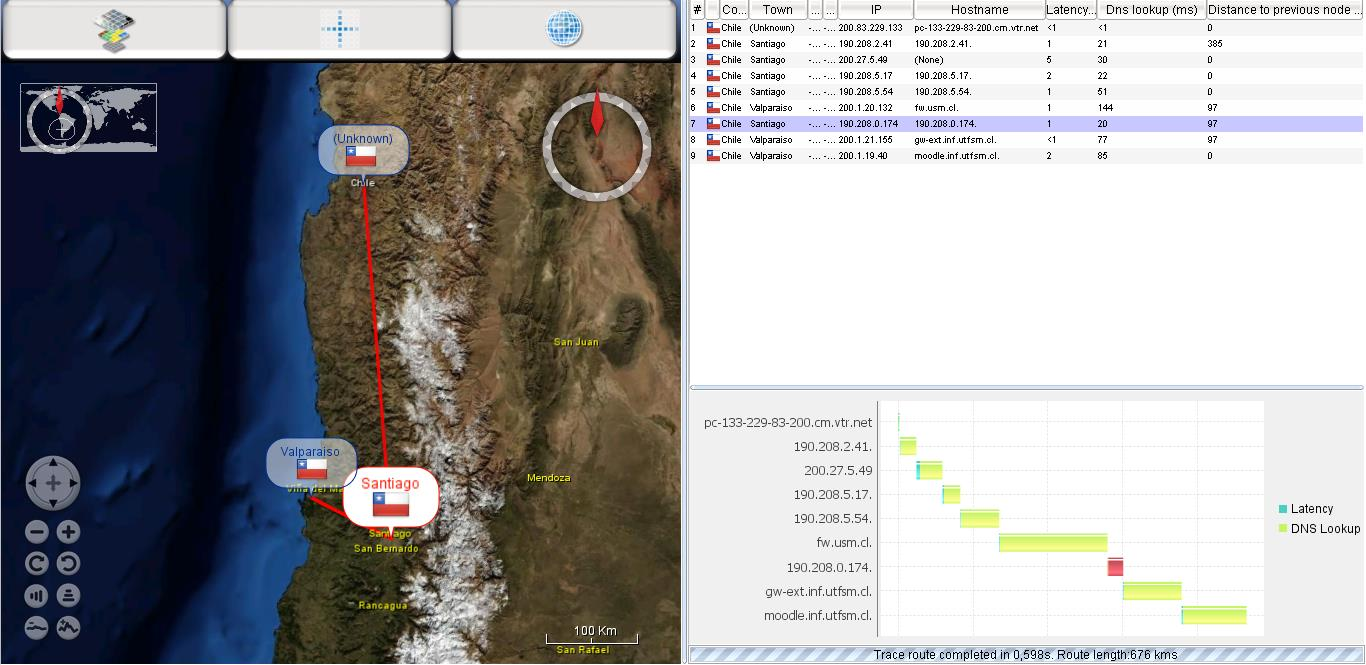
\includegraphics[width=0.8\textwidth]{./3.jpg}
  \caption{Traceroute efectuado a la web de Moodle}
  \label{fig:Traceroute efectuado a la web de Moodle}
\end{figure}
\begin{figure}
  \centering
    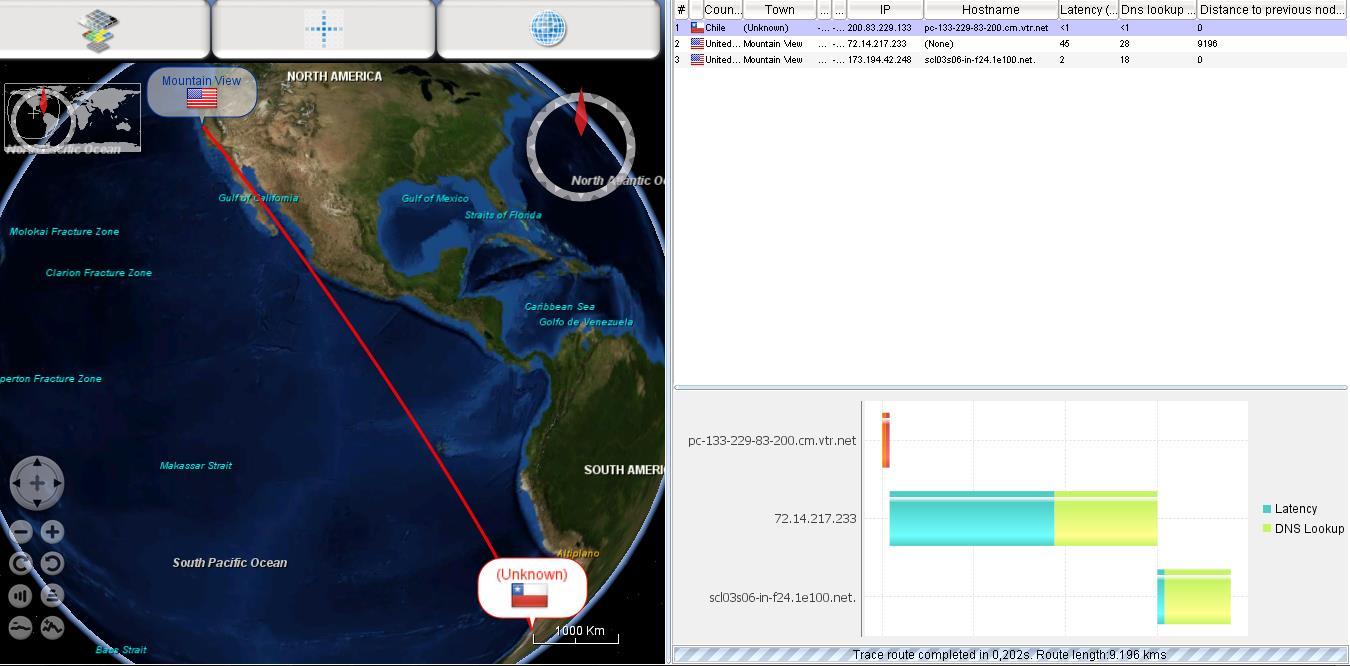
\includegraphics[width=0.8\textwidth]{./2.jpg}
  \caption{Traceroute efectuado a la web de Google}
  \label{fig:Traceroute efectuado a la web de Google}
\end{figure}
\begin{figure}
  \centering
    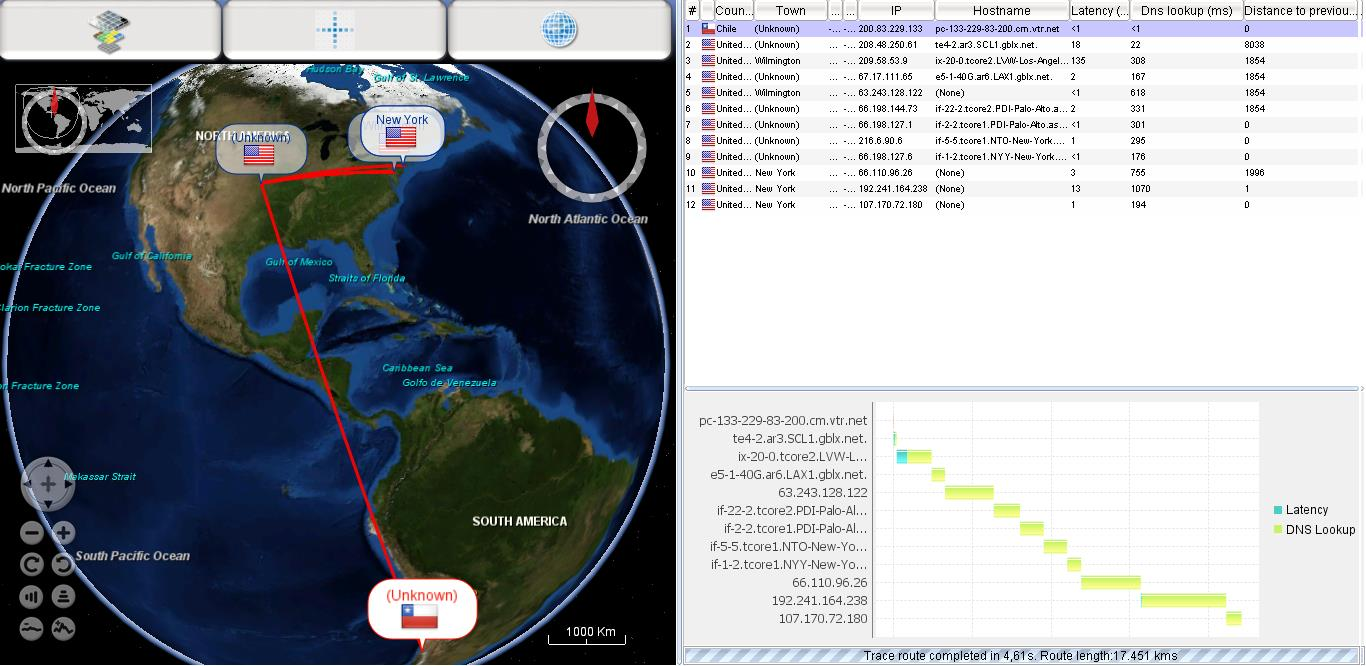
\includegraphics[width=0.8\textwidth]{./1.jpg}
  \caption{Traceroute efectuado a la web de CIME}
  \label{fig:Traceroute efectuado a la web de CIME}
\end{figure}
\begin{figure}
  \centering
    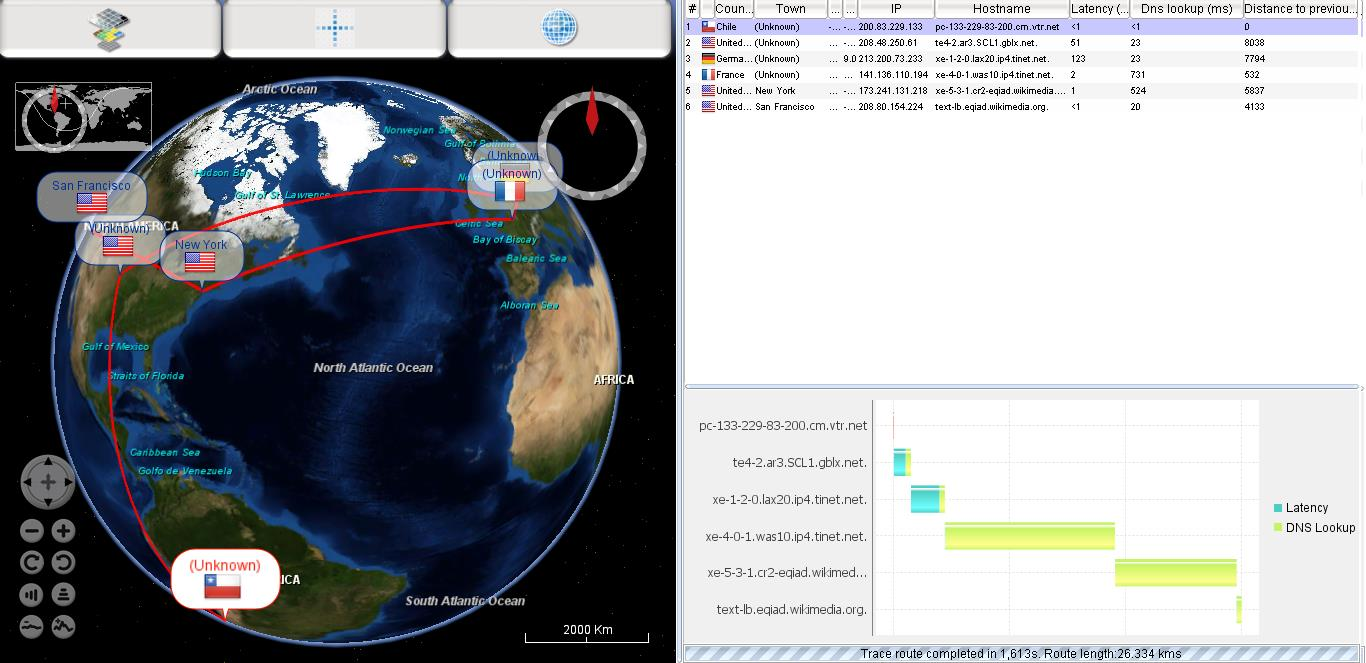
\includegraphics[width=0.8\textwidth]{./5.jpg}
  \caption{Traceroute efectuado a la web de Wikipedia}
  \label{fig:Traceroute efectuado a la web de Wikipedia}
\end{figure}
\begin{figure}
  \centering
    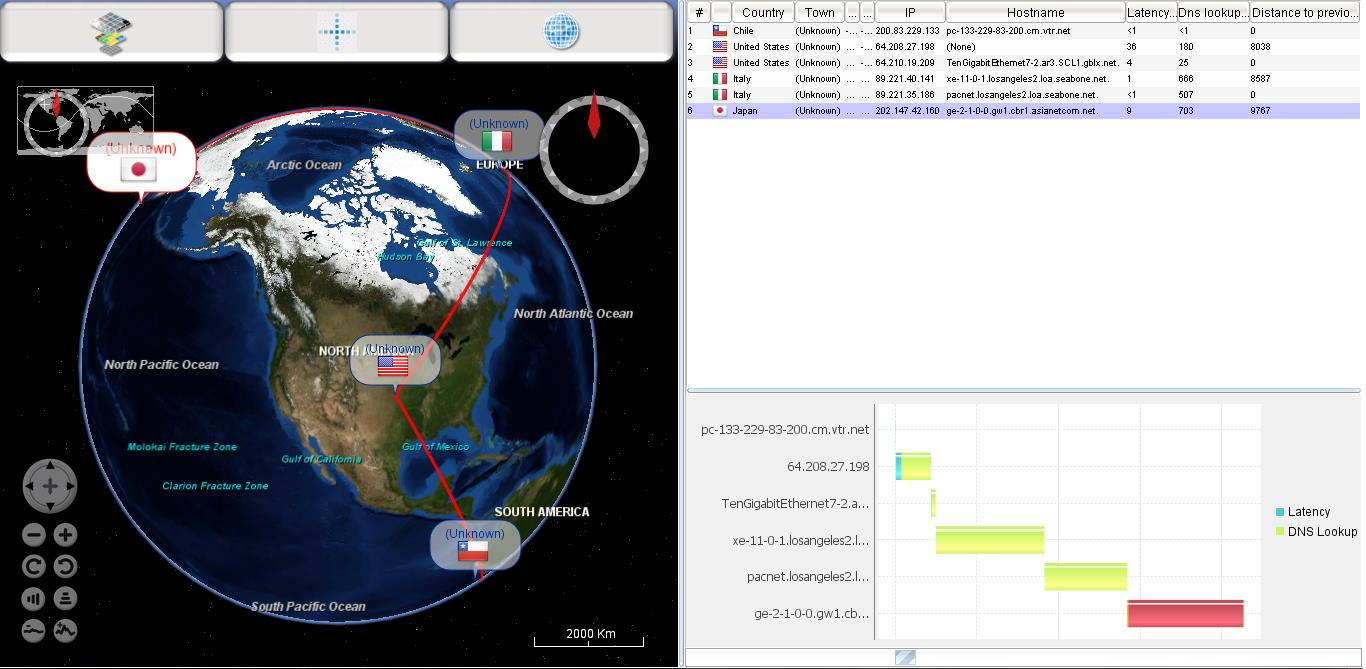
\includegraphics[width=0.8\textwidth]{./4.jpg}
  \caption{Traceroute efectuado a la web de Embajada}
  \label{fig:Traceroute efectuado a la web de Embajada}
\end{figure}

\end{document}